\section{Results}
We verify the estimation of the steady state execution time and energy consumption from the stage \textit{latency/energy estimation} in our framework. Table \ref{tab:est} summarizes the accuracy of our estimation for the streaming applications JPEG and MP3. We varied the number of tasks mapped on a PE and compared our estimations with the actual simulation. 

\begin{table}
{
\label{tab:est}
\begin{tabular}{|c|c|c|c|c|c|}
\hline
Benchmark &  Number of &\multicolumn{2}{|c}{Execution} & \multicolumn{2}{|c|}{Energy} \ \\
& tasks mapped & \multicolumn{2}{|c|}{Time}& \multicolumn{2}{|c|}{Consumption}\ \\
\hline
& & Max & Avg & Max & Avg\ \\
& & error & error & error & error\ \\
& & (\%) &  (\%) &  (\%) &  (\%)\ \\
\hline
\multirow{5}{*}{JPEG} &  1 & & & & \ \\
& 2 & & & & \\
& 3 & & & & \\
& 4 & & & & \\
& 5 & & & & \\
\hline
\multirow{5}{*}{MP3} &  1 & & & & \ \\
& 2 & & & & \\
& 3 & & & & \\
& 4 & & & & \\
& 5 & & & & \\
\hline
\end{tabular}
}
\end{table}

\begin{center}
\begin{table*}[ht]
{
\begin{tabular}{|c|c|c|c|c|c|c|c|}
\hline
 &  &\multicolumn{3}{|c|}{\textbf{Hierarchical Approach}} &  \multicolumn{3}{|c|}{\textbf{Ci x Ca x DVFS}}\\
%\cline{3-9}
\hline
Benchmark&Experiment &Maximum&Minimum& Average&Maximum&Minimum& Average\\
& Number & Improvement & Improvement & Improvement & Improvement & Improvement & Improvement\\
& & (\%) & (\%) & (\%) & (\%) & (\%) & (\%)\\ 
\hline
\multirow{2}{*}{JPEG} & 1 & 29.51 & 1.27 & 24.35 & 32.31 & 3.27 & 26.52\ \\
& 2 & 29.04 & 2.23 & 26.31 & 29.04 & 0.532 & 25.12 \ \\
\hline
\multirow{2}{*}{MP3} & 1 & 41.78 & 3.27 & 43.02 & 49.01 & 10.49 & 44.17\ \\
& 2 & 43.03 & 6.78 & 39.08 & 47.30 & 12.50 & 43.97 \ \\
\hline
\end{tabular}
}
\hfill{}
\caption{Experimental results in comparison with \textbf{Ci+Ca}}
\label{tb:comparison}
\end{table*}
\end{center}

%\begin{figure}[h]
%\center
%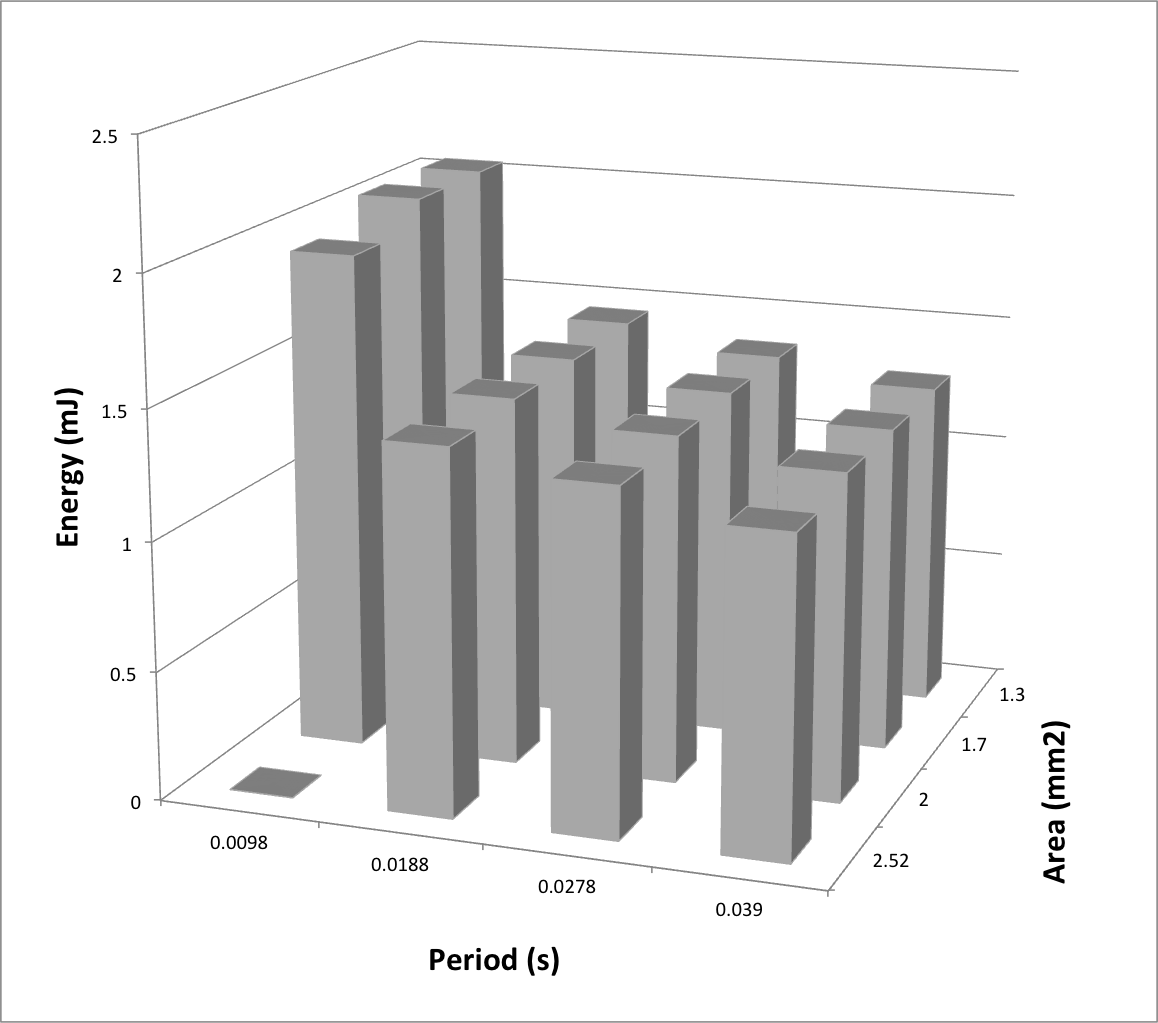
\includegraphics[width=0.36\textwidth]{CixCa+dvfs.png}
%\label{fig:CIxCa+dvfs}
%\caption {CixCa+DVFS for MP3}
%\end{figure}

%\begin{figure}[h]
%\center
%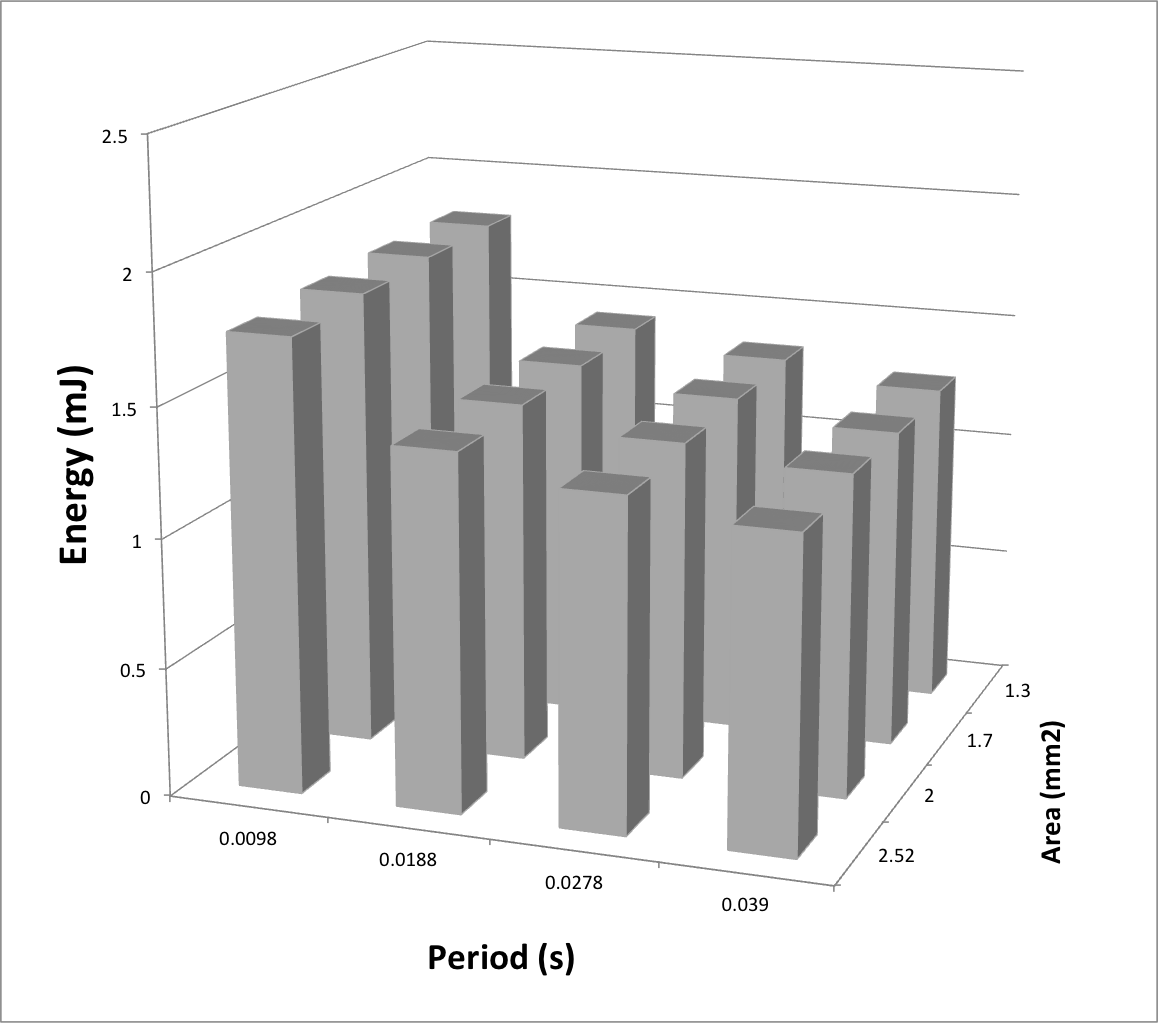
\includegraphics[width=0.36\textwidth]{CixCaxDVFS.png}
%\label{fig:CixCaxDVFS}
%\caption {CixCaxDVFS for MP3}
%\end{figure}
We compare the optimal points ASIP configuration obtained by the following techniques:
\begin{enumerate}
\item \textbf{CixCaxDVFS}: We use our branch and bound technique to find the optimal energy efficient ASIP configuration while modifying custom instruction set, cache configurations and voltage/frequency setting.
\item \textbf{CixCa+DVFS}: We call this technique as \textbf{Hierarchical Approach}. At the first stage, we optimize for the energy by only modifying custom instruction set and cache configurations. With the ASIP configuration obtained from the first stage, we apply different voltage/frequency setting to further reduce the energy. This technique can be derived by adding DVFS to the technique mentioned in \ref{}. 
\item \textbf{Ci+Ca}: Energy optimization by modifying only custom instruction set and cache configurations.
\end{enumerate}   

All the optimal points selected respects the input area and period constraints provided. As mentioned before, our design space consists of more than billion points along the axes of period, area and energy. Hence, it is not practical to plot all the points in a graph. Furthermore, we have two input constraints in terms of area and period. To get representative inputs for comparison, we perform two experiments per benchmark. In each of the experiments, we employ Latin hypercube sampling to generate 500 different tuples consisting of the area and period constraint. Using our branch and bound technique, we determine the lower bound of the period and the upper bound of the area by giving \textit{infinity} as an input constraint for both area and period for the target application. Similarly, the upper bound for the period is determined by summing the execution time of the software only versions of each task at the lowest possible cache configuration. The lowest bound for the area is equivalent to the size of a single PE and smallest cache configuration supported. With these bounds, latin hypercube sampling \ref{} efficiently covers the entire design space. 

We compare the results of the \textbf{CixCaxDVFS} and \textbf{CixCa+DVFS} with that of \textbf{Ci+Ca}. It is evident from the Table \ref{tb:comparison}, both the techniques significantly outperforms \textbf{Ci+Ca}. On an average, \textbf{CixCaxDVFS} performs better than \textbf{CixCa+DVFS}. This is because, the hierarchical nature of the technique \textbf{CixCa+DVFS} could result in the local optimum in comparison to the global optimum acheivable by \textbf{CixCaxDVFS}. Figure \ref{fig:CIxCa+dvfs} and \ref{fig:CIxCaxDVFS} shows the optimal energy acheivable for four different area and period constraint. In case of the hierarchical approach, we observed that there exists input constraints that was not satisfied to determine the optimal point. Thus, suggesting to consider all the three techniques (\textbf{Ci, Ca, DVFS} together. 